\subsection{Buck-boost converter}
\label{cap2-session-patino1}

    \comentarioblue{
        Atentar para sentencas que comecam com gerundio e nao terminam
    }

    \comentarioblue{
        Citar artigo do patino
    }
    
    \comentariopurple{
        convem que o tamanho e o tipo da font usada na figura seja
        igual ao do texto principal. Neste caso, seria conveniente 
        escrever E, L, C, R em italico. Tambem seria bom indicar a tensao
        vC e a corrent iL no circuito.
    }
    
    Considering a Buck-Boost converter in Continuous Conduction Mode (CCM) 
    which the topology is shown in Figure \refeq{cap2-circuit-ex-1}. 

    \begin{figure}[H]
        \centering
        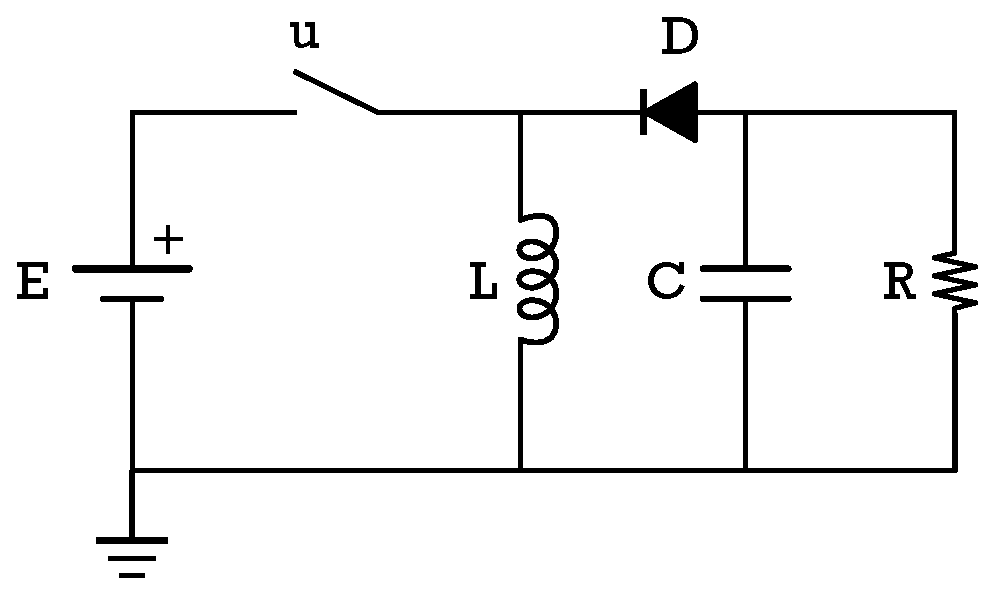
\includegraphics[width=10cm]{Cap2/fig/figura_circuito_ex_1.eps} 
        \caption{Buck-Boost converter}
        \label{cap2-circuit-ex-1}
    \end{figure}

    The state variables are the capacitor voltage \highlight{$v_c$} and the inductor current \highlight{$i_L$}. Its dynamics are given by the equation:

    \begin{equation}
        \dot{x} = \begin{cases}
            A_1 x + b_1\text{, for u = 1 (closed switch - Mode 1)} \\
            A_2 x + b_2\text{, for u = 0 (open switch - Mode 2)} 
        \end{cases}
    \end{equation}

    \noindent
    where

    \begin{equation}
        \label{eq_dynamics_patino1}
        \begin{matrix}
            A_1 = \left[ \begin{matrix} 0 & 0 \\ 0 & -\frac{1}{RC} \\ \end{matrix} \right] & 
            A_2 = \left[ \begin{matrix} 0 & \frac{1}{L} \\ -\frac{1}{C} & -\frac{1}{RC} \\ \end{matrix} \right] \\
            \\
            b_1 = \left[ \begin{matrix} \frac{E}{L} & 0 \end{matrix} \right]^T & 
            b_2 = \left[ \begin{matrix} 0 & 0 \end{matrix} \right]^T \\
        \end{matrix}
    \end{equation}

    \noindent
    where (in normalized values) \highlight{$R = L = C = E = 1$}. 

    The list of dynamics for this example is

    \noindent
    \begin{equation}
        \Big\{\big[A_1,b_1\big], \big[A_2,b_2\big]\Big\}
    \end{equation}

    \noindent
    where

    \noindent
    \begin{align}
        A_1 &= \left[
            \begin{matrix}
                0 & 0 \\ 
                0 & 1 \\ 
            \end{matrix}
        \right],
        b_1 = \left[
            \begin{matrix}
                0 \\ 
                1 \\ 
            \end{matrix}
        \right], \\
        A_2 &= \left[
            \begin{matrix}
                0 & 1 \\ 
                -1 & -1 \\ 
            \end{matrix}
        \right],
        b_2 = \left[
            \begin{matrix}
                0 \\ 
                0 \\ 
            \end{matrix}
        \right]
    \end{align}
    
    \comentarioblue{
        seria melhor fazer mencao ao custo em (2.2) e indicar que $\bar{x}^\infty = [2, -1]^T$
    }

    \comentarioblue{
        acho que tambem faltou mencionar a restricao de minimum dwell time. ela teria que ser formalizada
        em termos dos elementos $\tau^\infty$
    }

    \comentarioblue{
        acho que ficou faltando mensionar a restricao $T_p <= T_{p, max}$ na formulacao do problema de otimizacao
    }

    \comentarioblue{
        o uso de $dt$ ja precisaria ser explicado na formulacao do problema de otimizacao.
        talvez seja possivel aproveitar a discussar sobre o uso de $dt$ para introduzir a restricao 
        de minimum dwell time.
    }


    The criteria for the optimization is to compute the trajectory to minimize equation \eqref{cap2_eq_optimization} 
    with \highlight{$\bar{x}^\infty = \big[2, -1\big]^T$} with the weight matrix \highlight{$Q = diag\big[1,1\big]$}, the maximum cycle period of \highlight{$T_{p,max} = 1s$} and minimum 
    dwell time of \highlight{$t_{min} = 0.25s$}.

    The cost function takes a vector representing the \highlight{$dt$} for each switching moment as its 
    input. For instance, with two switching instances, the vector could be \highlight{$\big[ 0.25, 0.35\big]$}. 
    This implies the signal begins at time \highlight{$0.0$}, transitions to the next 
    dynamic at \highlight{$0.0 + 0.25 = 0.25$}, and then switches again at \highlight{$0.25 + 0.35 = 0.6$}. This gives us the signal sequence 
    \highlight{$\big[0.0, 0.25, 0.6\big]$}.

    In the Buck-Boost converter example, the initial values for the switching vector are represented 
    by \highlight{$[0.25, 0.25]$}. The lower bounds are defined as \highlight{$[0.25, 0.25]$} and the upper bounds 
    are set to \highlight{$[1.5, 1.5]$}. The solution provided by the \highlight{FMINCON} optimization yields 

    \begin{equation}
        \label{eq_ref_signal_patino1}
        \begin{matrix}
            \tau^\infty = \big[0, 0.2513, 0.5914\big],\\
            \\
            \Omega^\infty = \big[1, 2\big].
        \end{matrix}
    \end{equation}

    \comentariopurple{
        nao usar parenteses na numeracao d figuras
    }

    The outcome under this condition is displayed in Figure \ref{cap2-graf-ex1-1}, showcasing 
    the cyclic trajectory around the average value \highlight{$[2, -1]^T$}. The corresponding switch command signal $u$ 
    can be seen in Figure \ref{cap2-graf-ex1-2}.

    \comentarioblue{
        usar $x_1$ e $x_2$ nos labels dos eixos da figura
    }

    \begin{figure}[h]
        \centering
        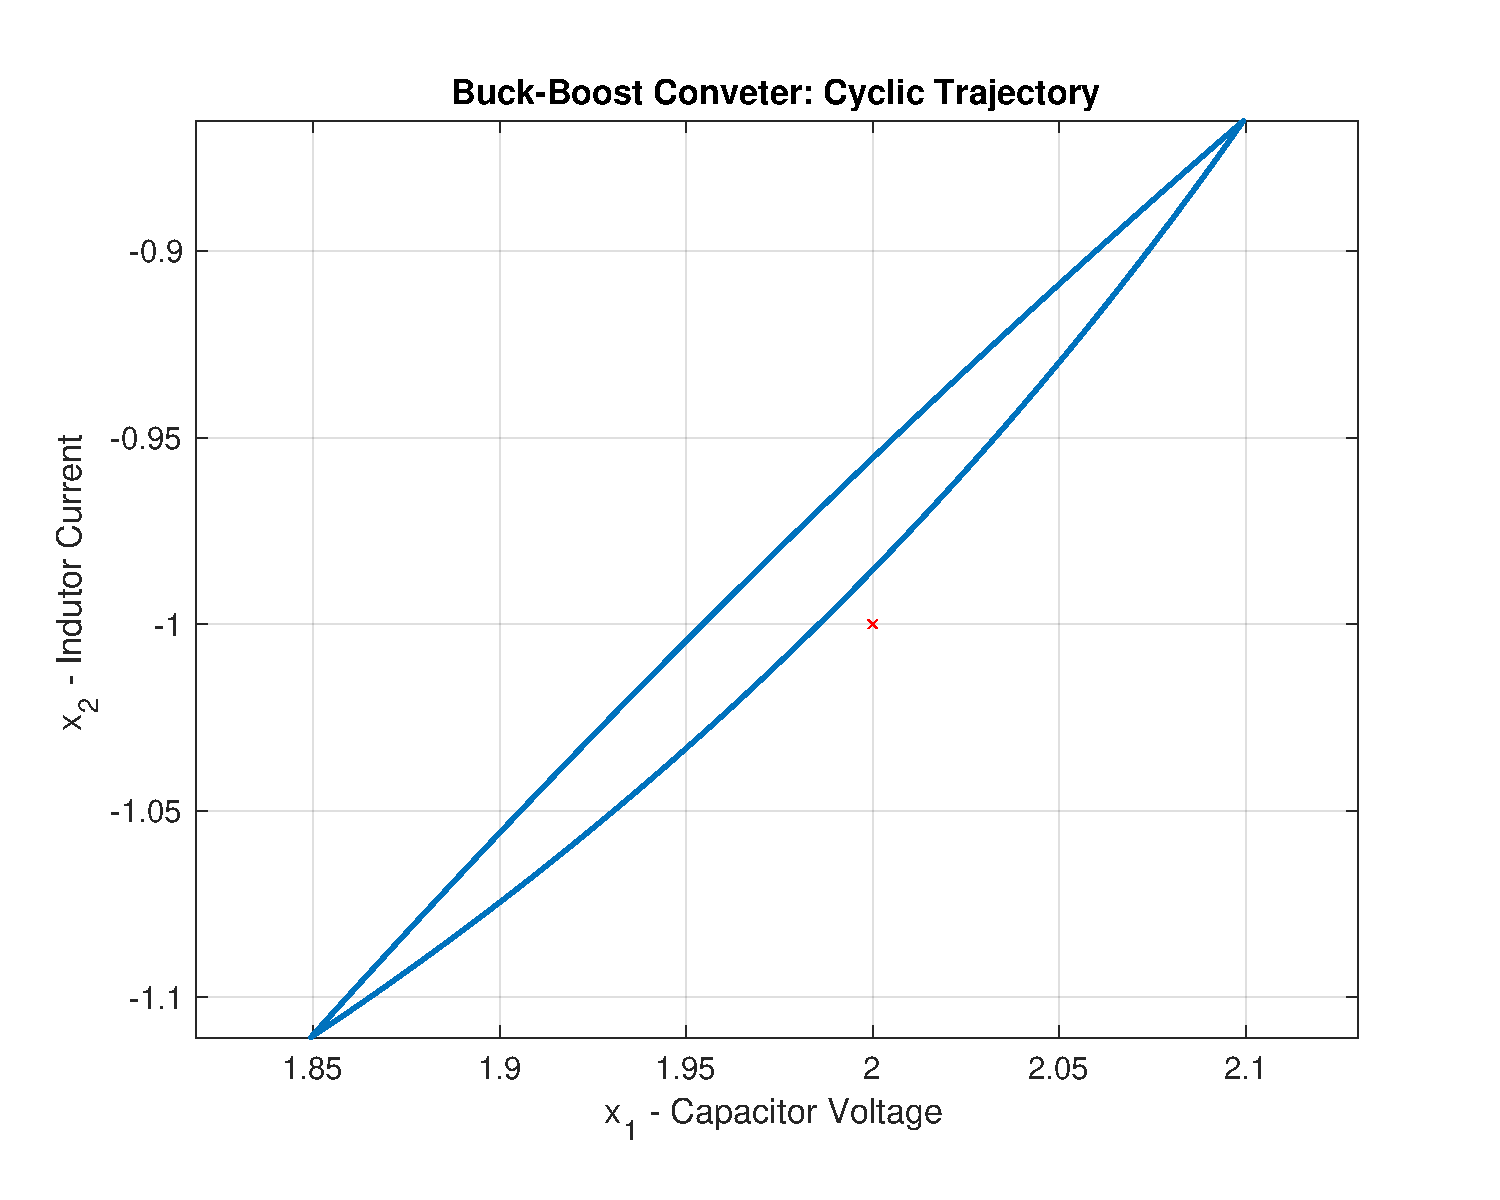
\includegraphics[width=14cm]{Cap2/fig/graf_ex1_1.pdf}
        \caption{Buck-Boost converter: State trajectory}
        \label{cap2-graf-ex1-1}
    \end{figure}

    \comentarioblue{
        xlabel: u - switch command
    }

    \begin{figure}[H]
        \centering
        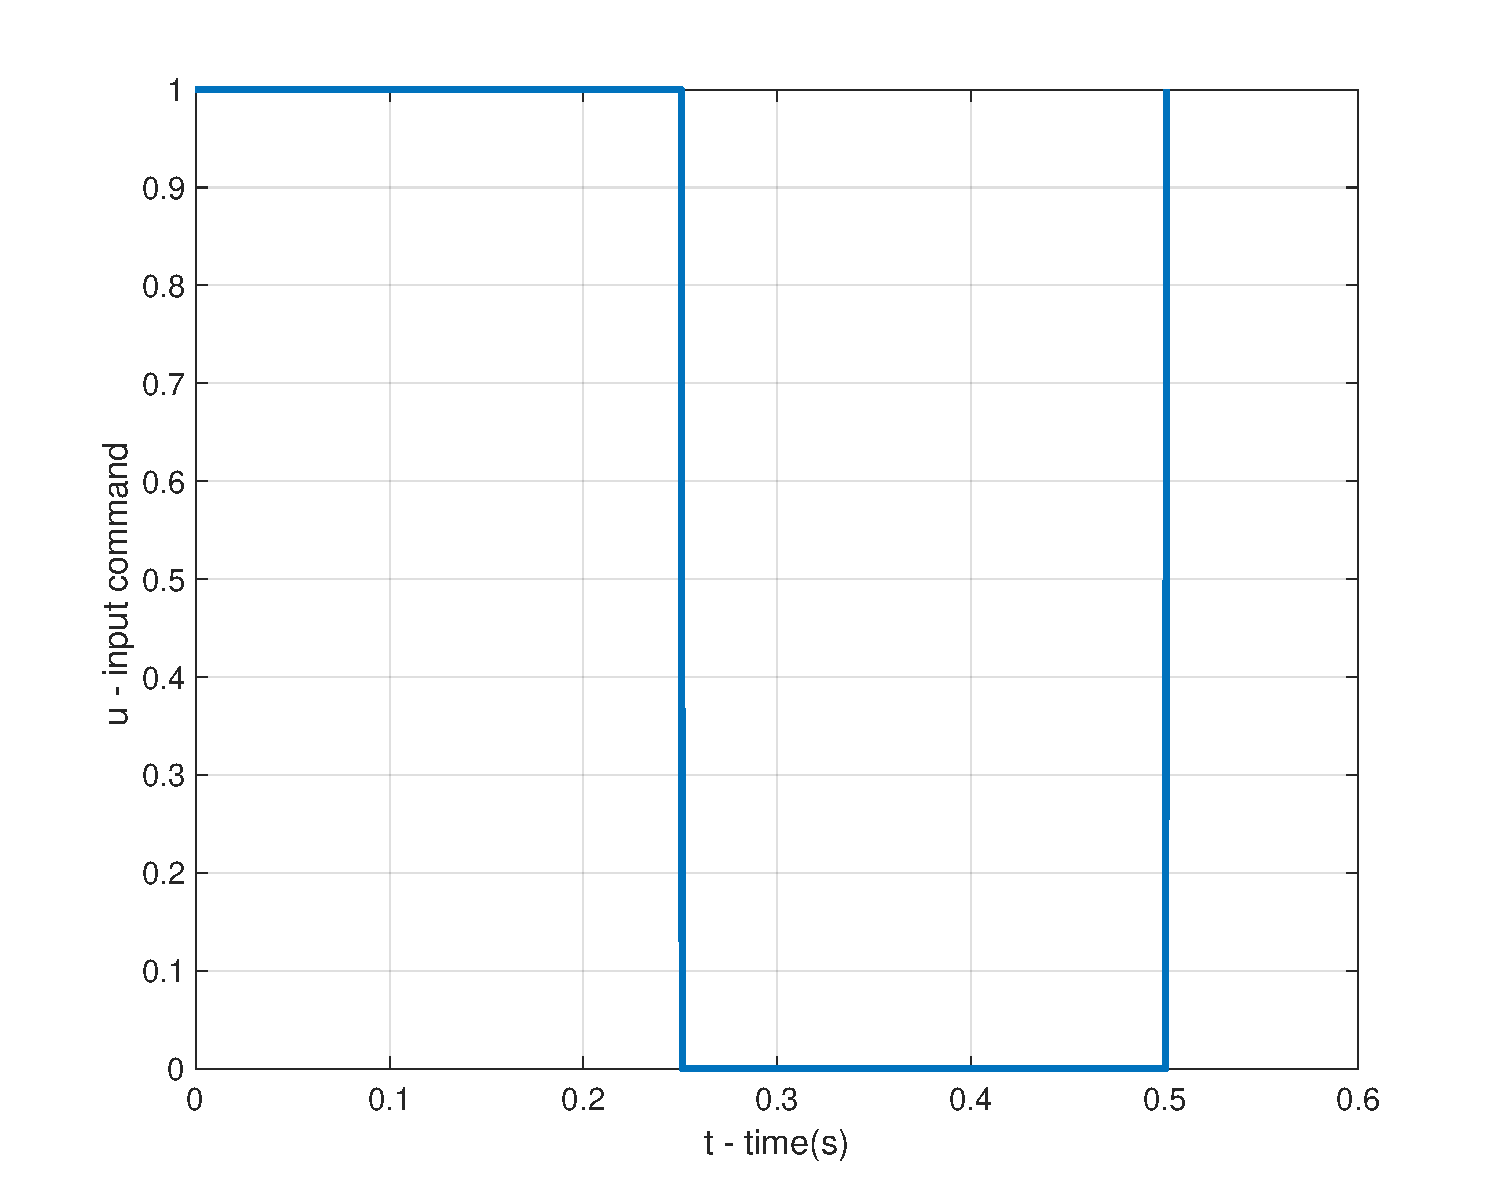
\includegraphics[width=14cm]{Cap2/fig/graf_ex1_2.pdf}
        \caption{Buck-Boost converter: Switch command}
        \label{cap2-graf-ex1-2}
    \end{figure}